\documentclass[11pt,a4paper]{article}
\usepackage[margin=2.2cm]{geometry}
\usepackage{graphicx}
\usepackage{booktabs}
\usepackage{amsmath,amssymb}
\usepackage{siunitx}
\usepackage{xcolor}
\usepackage[colorlinks=true,linkcolor=blue!60!black,citecolor=green!50!black]{hyperref}
\usepackage{caption}
\usepackage{subcaption}
\usepackage{float}

\definecolor{boxblue}{RGB}{230,242,255}
\definecolor{boxamber}{RGB}{255,243,224}
\definecolor{boxgreen}{RGB}{232,245,233}

\graphicspath{{figures/}}

\title{Bayesian Identifiability Analysis of Europa's Ice Shell\\
\large Posterior Covariance, Information Ladder, and Shapley Effects\\[4pt]
\normalsize Under the Juno MWR Conductive-Lid Constraint ($D_\mathrm{cond} = 29 \pm \SI{10}{\kilo\metre}$)\\[2pt]
\normalsize Global Andrade Baseline (\texttt{mc\_15000\_optionA\_v2\_andrade})}

\author{EuropaConvection Project --- Generated \today}
\date{}

\begin{document}
\maketitle

% ======================================================================
\section{Executive Summary}
% ======================================================================

\fcolorbox{blue!30}{boxblue}{\parbox{0.96\textwidth}{%
The Juno MWR conductive-lid constraint provides \textbf{weak information}
($\mathrm{KL} = 0.103$~nats, ESS/$N = 83.6\%$, PSIS $\hat{k} = -1.30$
indicating a bounded, reliably-sampled tail).  The prior ensemble is in
\textbf{mild tension} with the observation: only $0.21\%$ of prior samples
have $D_\mathrm{cond} \geq 29$~km, which the reweight doubles to $0.43\%$.
The posterior predictive median shifts from $16.0$~km (prior) to $17.7$~km
against a likelihood width of $\sigma_\mathrm{eff} = 10.4$~km.  No single
parameter is strongly identified: marginal shrinkages are all $\leq 5\%$.
A genuine restricted-update ladder (kNN-based conditional-mean emulation of
$L_S(\theta_S) = E_{\theta_{-S}}[L(\theta)]$) shows the information
\textbf{concentrated on two parameters}: $\varepsilon_0$ alone recovers
$51\%$ of the full posterior KL, and $\varepsilon_0 + q_\mathrm{basal}$
together recover $69\%$.  Adding any third parameter produces no further gain
within estimator noise.  \textbf{Verdict: H2 --- two-parameter restricted
identifiability on $\varepsilon_0$ and $q_\mathrm{basal}$}, with the
remaining three parameters uninformed by Juno.  The overall regime is
\emph{weak-to-moderate}: the information is structured but of small absolute
magnitude.
}}

\vspace{1em}

% ======================================================================
\section{Methodology}
% ======================================================================

\subsection{Competing Hypotheses}

Four mutually exclusive outcomes were defined \emph{a priori} with quantitative
thresholds (Table~\ref{tab:thresholds}):

\begin{description}
\item[H1: Single-parameter dominance] One parameter shrinks $>$50\%; others $<$10\%.
\item[H2: Trade-off manifold] Weak marginal shrinkage ($<$30\% each) but strong
  posterior correlation ($|r| > 0.5$) or a single dominant eigenvalue direction.
\item[H3: Weak information] All shrinkage $<$10\%, $\mathrm{KL} < 0.05$~nats.
\item[H4: Hierarchical identifiability] Monotonically decreasing shrinkage with
  eigenvalue spectrum spanning $>$1 order of magnitude.
\end{description}

\begin{table}[h]
\centering
\caption{A priori decision thresholds (declared before examining results).}
\label{tab:thresholds}
\begin{tabular}{lcccc}
\toprule
Metric & Negligible & Weak & Moderate & Strong \\
\midrule
Marginal shrinkage & $<$10\% & 10--30\% & 30--60\% & $>$60\% \\
Posterior $|r|$ & $<$0.2 & 0.2--0.5 & 0.5--0.7 & $>$0.7 \\
Eigenvalue $\rho_i$ & $>$0.9 & 0.5--0.9 & 0.1--0.5 & $<$0.1 \\
KL divergence (nats) & $<$0.05 & 0.05--0.2 & 0.2--1.0 & $>$1.0 \\
\bottomrule
\end{tabular}
\end{table}

\subsection{Three Complementary Methods}

\begin{enumerate}
\item \textbf{Prior-normalized eigenanalysis} of
  $R = \Sigma_\mathrm{prior}^{-1/2}\,\Sigma_\mathrm{post}\,\Sigma_\mathrm{prior}^{-1/2}$.
  Eigenvalues $\rho_i < 0.5$: data-informed; $\rho_i > 0.9$: prior-dominated.
\item \textbf{Restricted-update ladder}: for each subset $S$ of parameters we
  compute the restricted posterior $p_S(\theta_S \mid D) \propto p_S(\theta_S) \,
  L_S(\theta_S)$, where the marginalised likelihood
  $L_S(\theta_S) = \mathbb{E}_{\theta_{-S} \sim \mathrm{prior}}[L(\theta)]$ is
  estimated nonparametrically via a kNN conditional-mean emulator on the
  $z$-scored $|S|$-dimensional subspace
  ($k = \max(50,\ \sqrt{N}) \approx 122$ for $N = 14\,999$).  The greedy
  forward-selection ladder at each step adds the parameter whose inclusion
  maximises the resulting restricted KL.  This replaces an earlier
  implementation that returned the full joint-posterior weights for every
  subset (rendering the ``ladder'' a marginal ranking); the current results
  use the genuine restricted update.
\item \textbf{Shapley effects (exploratory attribution)}: binned
  conditional-variance estimates on SIR-resampled posterior draws that
  approximate a Shapley variance decomposition of $D_\mathrm{cond}$ (following
  Owen 2014; Song, Nelson, Staum 2016).  These values are reported as relative
  attribution, not as a definitive identifiability proof.
\end{enumerate}

\subsection{Baseline and Likelihood}

The analysis uses the global Andrade Monte Carlo ensemble
(\texttt{mc\_15000\_optionA\_v2\_andrade.npz}, $N = 14\,999$ valid samples).
Five physical parameters are varied: basal heat flux $q_\mathrm{basal}$,
grain size $d_\mathrm{grain}$, viscosity activation energy $Q_v$, tidal
reference strain $\varepsilon_0$ (Beuthe~2013 eccentricity-tide pattern),
and surface temperature $T_\mathrm{surf}$.  The Juno MWR likelihood is
$\mathcal{N}(\mu = 29\,\mathrm{km},\ \sigma_\mathrm{eff} = 10.4\,\mathrm{km})$
with $\sigma_\mathrm{eff} = \sqrt{\sigma_\mathrm{obs}^2 + \sigma_\mathrm{model}^2}$
combining the Levin et~al.~2026 observational uncertainty
($\sigma_\mathrm{obs} = 10$~km) with a model-discrepancy term
($\sigma_\mathrm{model} = 3$~km).  Posterior weights are computed by
importance sampling with stabilised log-likelihoods.

\subsection{Prior Predictive Check}

Before the identifiability analysis, the prior ensemble must be compared to the
Juno central value.  The prior predictive distribution of $D_\mathrm{cond}$ has
median $16.0$~km and $68\%$ CI $[11.7, 20.0]$~km --- the Juno central value of
$29$~km lies in the right tail of the prior:

\begin{table}[H]
\centering
\caption{Prior predictive mass at and above the Juno central value.}
\label{tab:priortension}
\begin{tabular}{lcc}
\toprule
Quantity & Prior & Posterior \\
\midrule
Median $D_\mathrm{cond}$ (km) & 16.0 & 17.7 \\
68\% CI (km) & [11.7, 20.0] & [14.0, 21.6] \\
$P(D_\mathrm{cond} \geq 29\,\mathrm{km})$ & $0.21\%$ & $0.43\%$ \\
$P(D_\mathrm{cond} \geq 19\,\mathrm{km})$ & $\sim 21\%$ & $\sim 31\%$ \\
\bottomrule
\end{tabular}
\end{table}

\textbf{Prior/observation tension.} The prior ensemble places almost no mass at
the Juno central value: only $0.21\%$ of prior samples sit at or above $29$~km.
Importance-sampling reweighting doubles that to $0.43\%$, but the bulk of the
posterior still lives well below the Juno central value.  This is a structural
feature of the prior/forward-model combination, not a bug in the weighting code:
Juno is \emph{compatible} with the prior (the observation sits $\sim 1.3\sigma$
from the prior median of $\sim 16$~km under $\sigma_\mathrm{eff} = 10.4$~km),
but only in the prior's extreme tail.  Any identifiability conclusion drawn
from this posterior should be read in that light --- the data cannot move the
posterior median meaningfully closer to $29$~km without invoking tail samples
that have near-zero prior weight.

% ======================================================================
\section{Phase 1: Posterior Covariance and Identifiability}
% ======================================================================

\subsection{Summary Statistics}

\begin{table}[H]
\centering
\caption{Headline diagnostics for the global Andrade baseline.}
\label{tab:phase1}
\begin{tabular}{lc}
\toprule
Metric & Global Andrade baseline \\
\midrule
$N$ (prior samples) & 14\,999 \\
ESS (Kish) & 12\,541 (83.6\%) \\
$\mathrm{KL}(\mathrm{post}\|\mathrm{prior})$ & 0.103~nats [0.101, 0.105] \\
Leading $\rho_1$ & 0.821 [0.802, 0.838] \\
$\varepsilon_0$ shrinkage & $+$2.7\% [0.8, 4.7] \\
$q_\mathrm{basal}$ shrinkage & $-$4.7\% \\
$Q_v$ shrinkage & $-$2.2\% \\
$d_\mathrm{grain}$ shrinkage & $-$1.5\% \\
$T_\mathrm{surf}$ shrinkage & $-$0.8\% \\
Strongest posterior correlation & $q_\mathrm{basal}$--$\varepsilon_0$: $+$0.18 \\
\bottomrule
\end{tabular}
\end{table}

\paragraph{Reading the shrinkage values.}
Only $\varepsilon_0$ shows positive marginal shrinkage with a 95\% CI that
excludes zero ($+2.7\%$ [$+0.8$, $+4.7$]).  The remaining four parameters
show slightly negative point estimates; these reflect Monte Carlo sampling
noise around zero shrinkage (the posterior marginals are statistically
indistinguishable from the prior marginals at $N_\mathrm{eff} \approx 12\,500$),
not a literal widening of the posterior.  No parameter reaches even the
10\% ``negligible'' threshold declared \emph{a priori}.

\subsection{Prior-Normalized Eigenanalysis}

\begin{figure}[H]
\centering
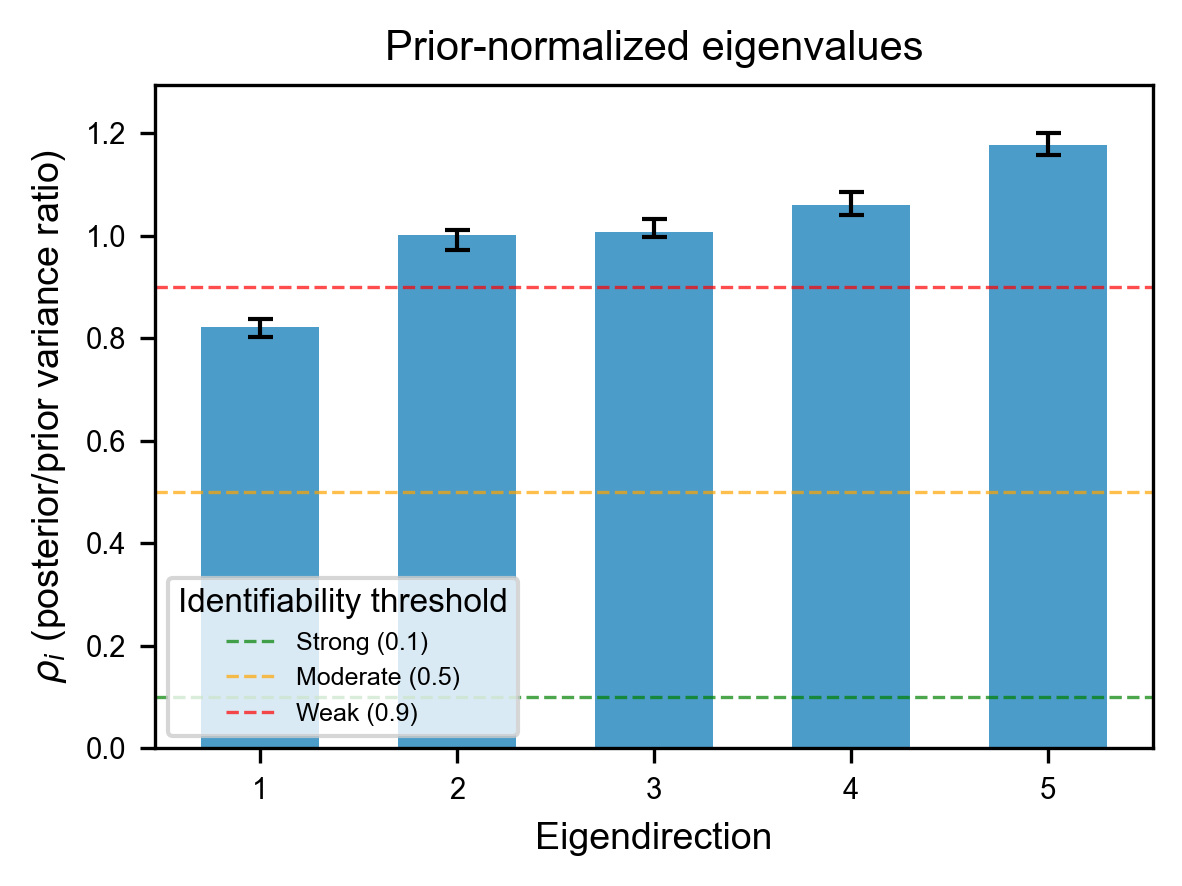
\includegraphics[width=0.7\textwidth]{global_andrade_scree_plot.png}
\caption{Prior-normalized eigenvalues $\rho_i$ of $R$ with bootstrap 95\% CIs.
  Only direction~1 ($\rho_1 = 0.82$) crosses the weak-identifiability threshold
  (red dashed line).  Directions 2--5 sit at or above $\rho = 1$, i.e.~the
  posterior variance along those axes is statistically indistinguishable from
  (or marginally looser than) the prior variance --- consistent with no information
  gain in those directions.}
\label{fig:scree}
\end{figure}

\begin{figure}[H]
\centering
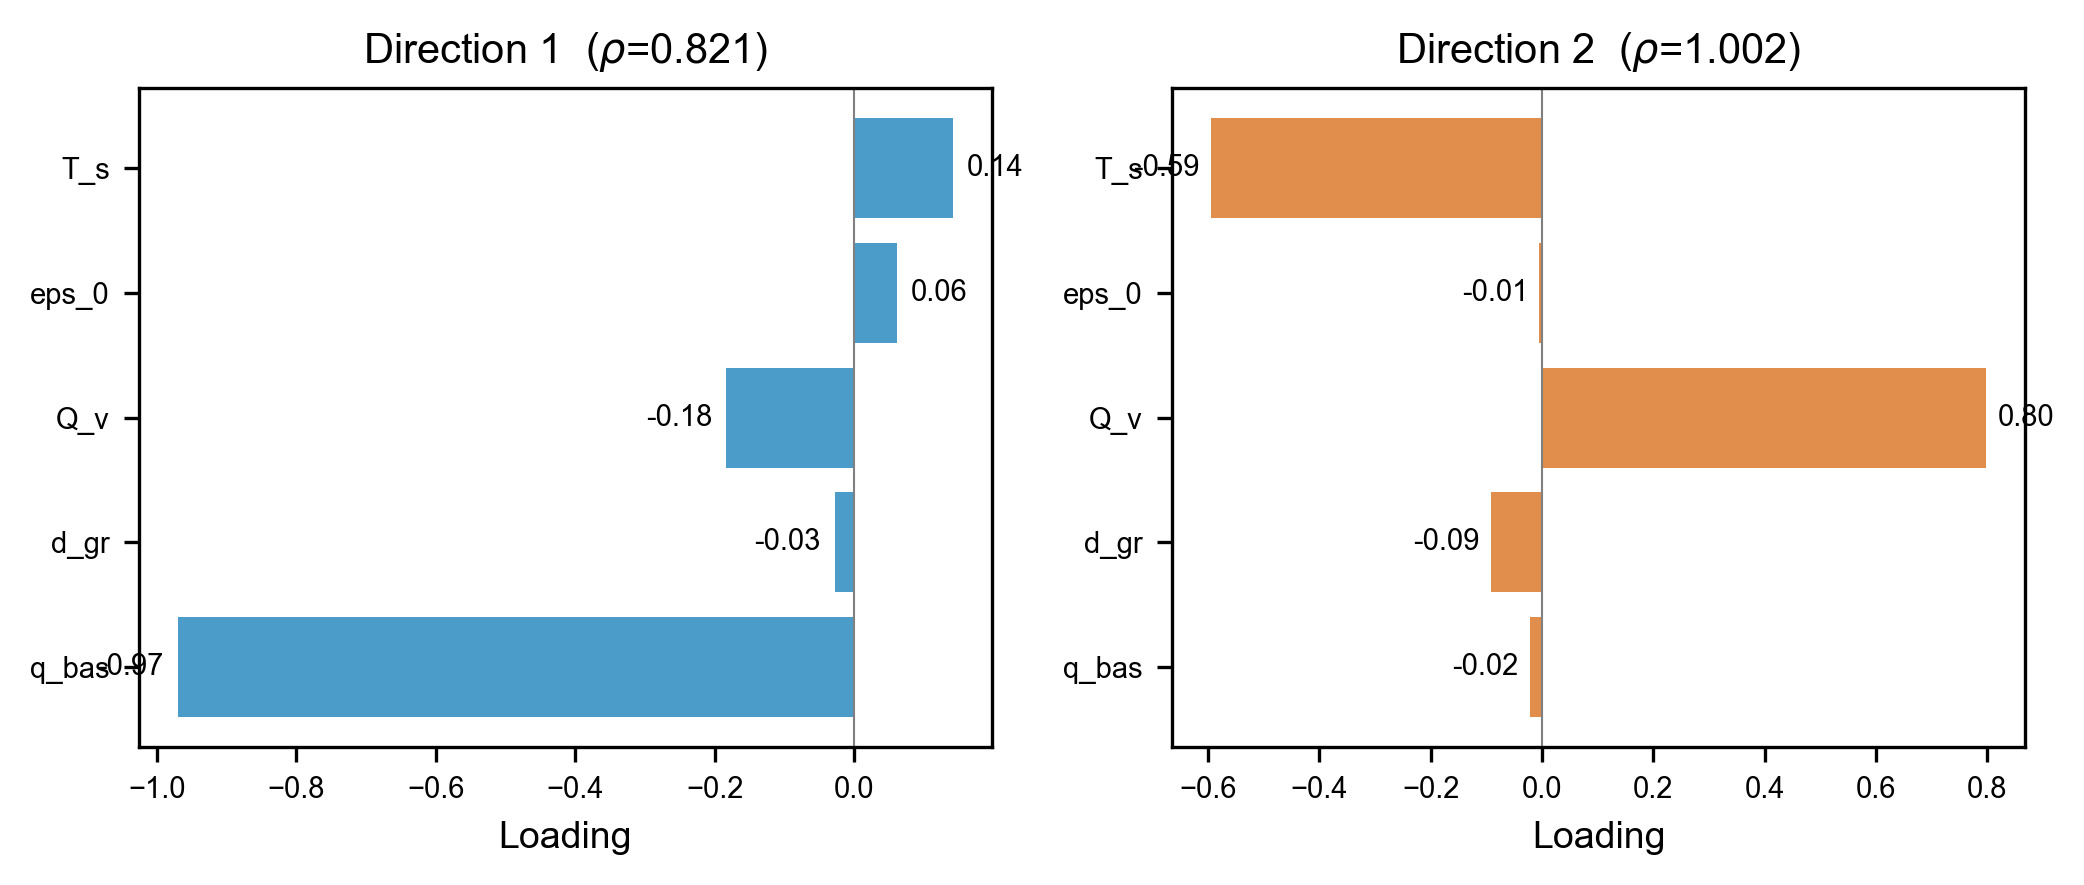
\includegraphics[width=0.95\textwidth]{global_andrade_loading_plot.png}
\caption{Eigenvector loadings for the two lowest-$\rho$ directions.
  Direction~1 ($\rho_1 = 0.82$, weakly informed) is dominated by
  $q_\mathrm{basal}$ ($-0.97$) with secondary $Q_v$ ($-0.18$) and
  $T_\mathrm{surf}$ ($+0.14$) contributions --- Juno's only compression
  of the posterior is along a combination that is essentially $q_\mathrm{basal}$.
  Direction~2 ($\rho_2 \approx 1.00$, uninformed) is a $Q_v$--$T_\mathrm{surf}$
  trade-off left unchanged by the observation.}
\label{fig:loadings}
\end{figure}

\paragraph{The marginal--eigenvector split.}
A subtlety of the global Andrade result: the largest \emph{marginal} information
gain sits on $\varepsilon_0$, but the largest \emph{posterior-geometry}
compression sits along the $q_\mathrm{basal}$ axis.  These are not contradictory.
The marginal ladder measures how much the posterior density for each parameter
moves relative to its prior; the eigenanalysis measures the direction of largest
variance reduction in the joint posterior covariance.  Juno updates $\varepsilon_0$'s
marginal directly, while the induced $q_\mathrm{basal}$--$\varepsilon_0$
correlation ($r = +0.18$) is what produces the $q_\mathrm{basal}$-dominated
eigendirection.

\subsection{Shrinkage and Correlations}

\begin{figure}[H]
\centering
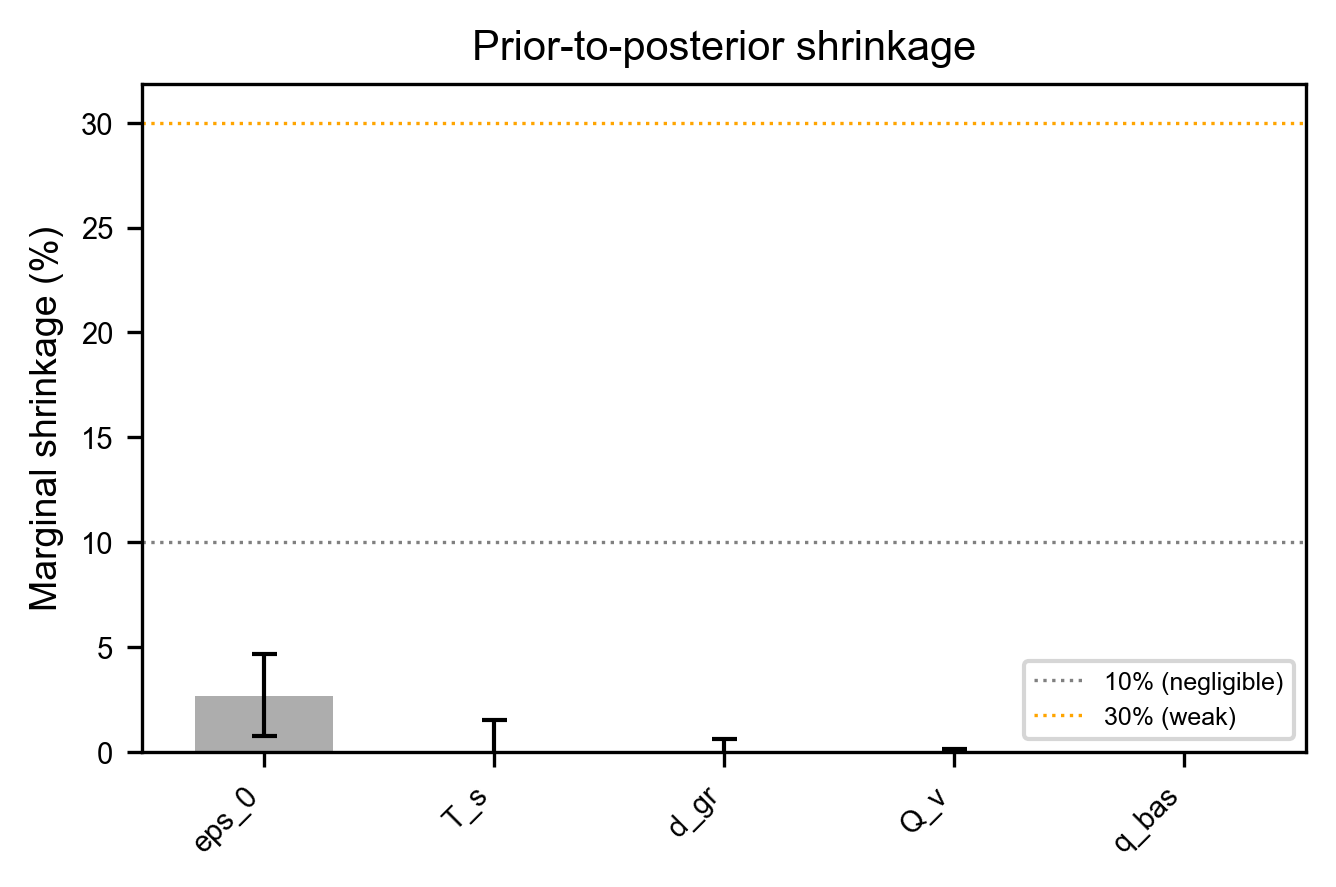
\includegraphics[width=0.75\textwidth]{global_andrade_shrinkage_waterfall.png}
\caption{Marginal prior-to-posterior shrinkage with bootstrap 95\% CIs.
  Only $\varepsilon_0$ exceeds zero at 95\% confidence, at $+2.7\%$ --- well
  below the 10\% ``negligible'' threshold.  The remaining parameters are
  consistent with zero shrinkage.}
\label{fig:shrinkage}
\end{figure}

\begin{figure}[H]
\centering
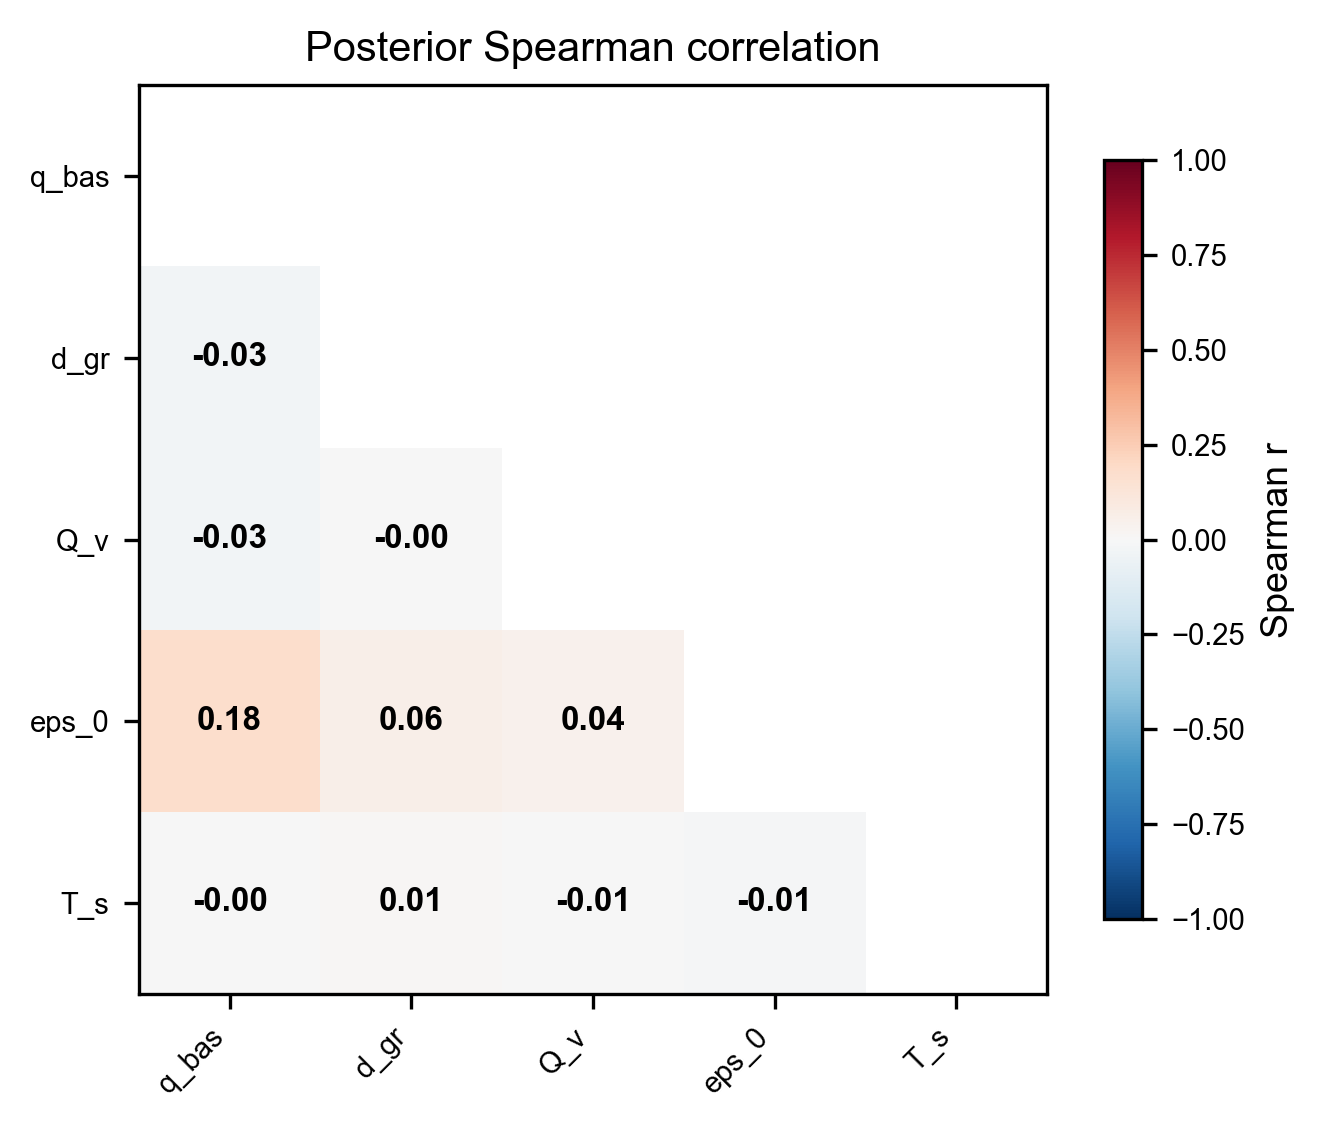
\includegraphics[width=0.6\textwidth]{global_andrade_correlation_heatmap.png}
\caption{Posterior Spearman correlation matrix.  No pair exceeds the 0.2
  threshold.  The largest value ($q_\mathrm{basal}$--$\varepsilon_0$,
  $r = +0.18$) is the induced trade-off that produces the single weak
  eigendirection; all other cross-correlations are $|r| < 0.07$.}
\label{fig:corr}
\end{figure}

\begin{figure}[H]
\centering
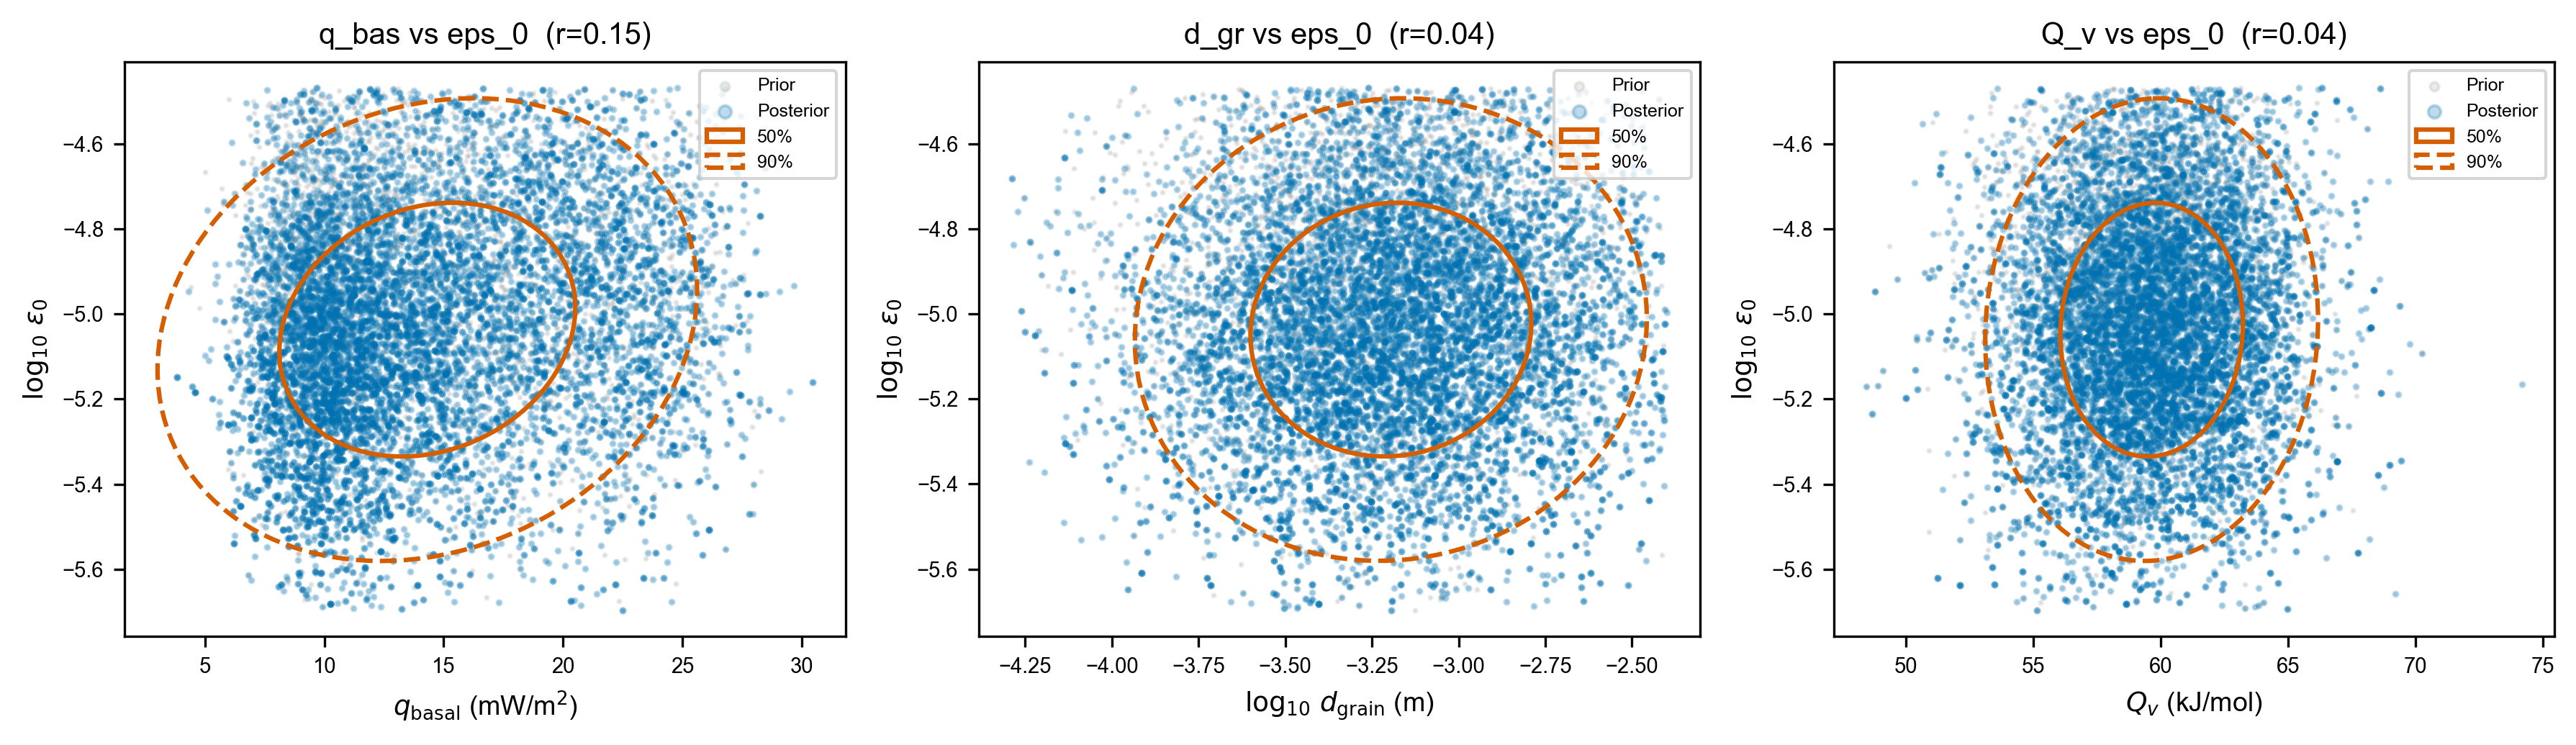
\includegraphics[width=0.95\textwidth]{global_andrade_pair_plot.png}
\caption{Prior (blue) vs posterior (orange contours) scatter for
  $\varepsilon_0$ paired with $q_\mathrm{basal}$, $d_\mathrm{grain}$, and $Q_v$.
  Orange ellipses: 50\% and 90\% credible regions.  The 90\% contours lie
  almost exactly on the prior cloud --- Juno tightens $\varepsilon_0$'s marginal
  slightly, but does not produce visible joint-density structure with any other
  parameter.}
\label{fig:pairs}
\end{figure}

% ======================================================================
\section{Phase 2: Restricted-Update Ladder}
% ======================================================================

For each subset $S$, the posterior is refit with the likelihood marginalised
over parameters outside $S$ using the kNN conditional-mean emulator described
in \S2.2.  The resulting KL divergence measures how much information Juno
\emph{could} supply if only the parameters in $S$ were allowed to update.
Row-level diagnostics (ESS, shrinkage, medians) reflect each restricted
posterior separately.

\subsection{Information Accumulation Curve}

\begin{figure}[H]
\centering
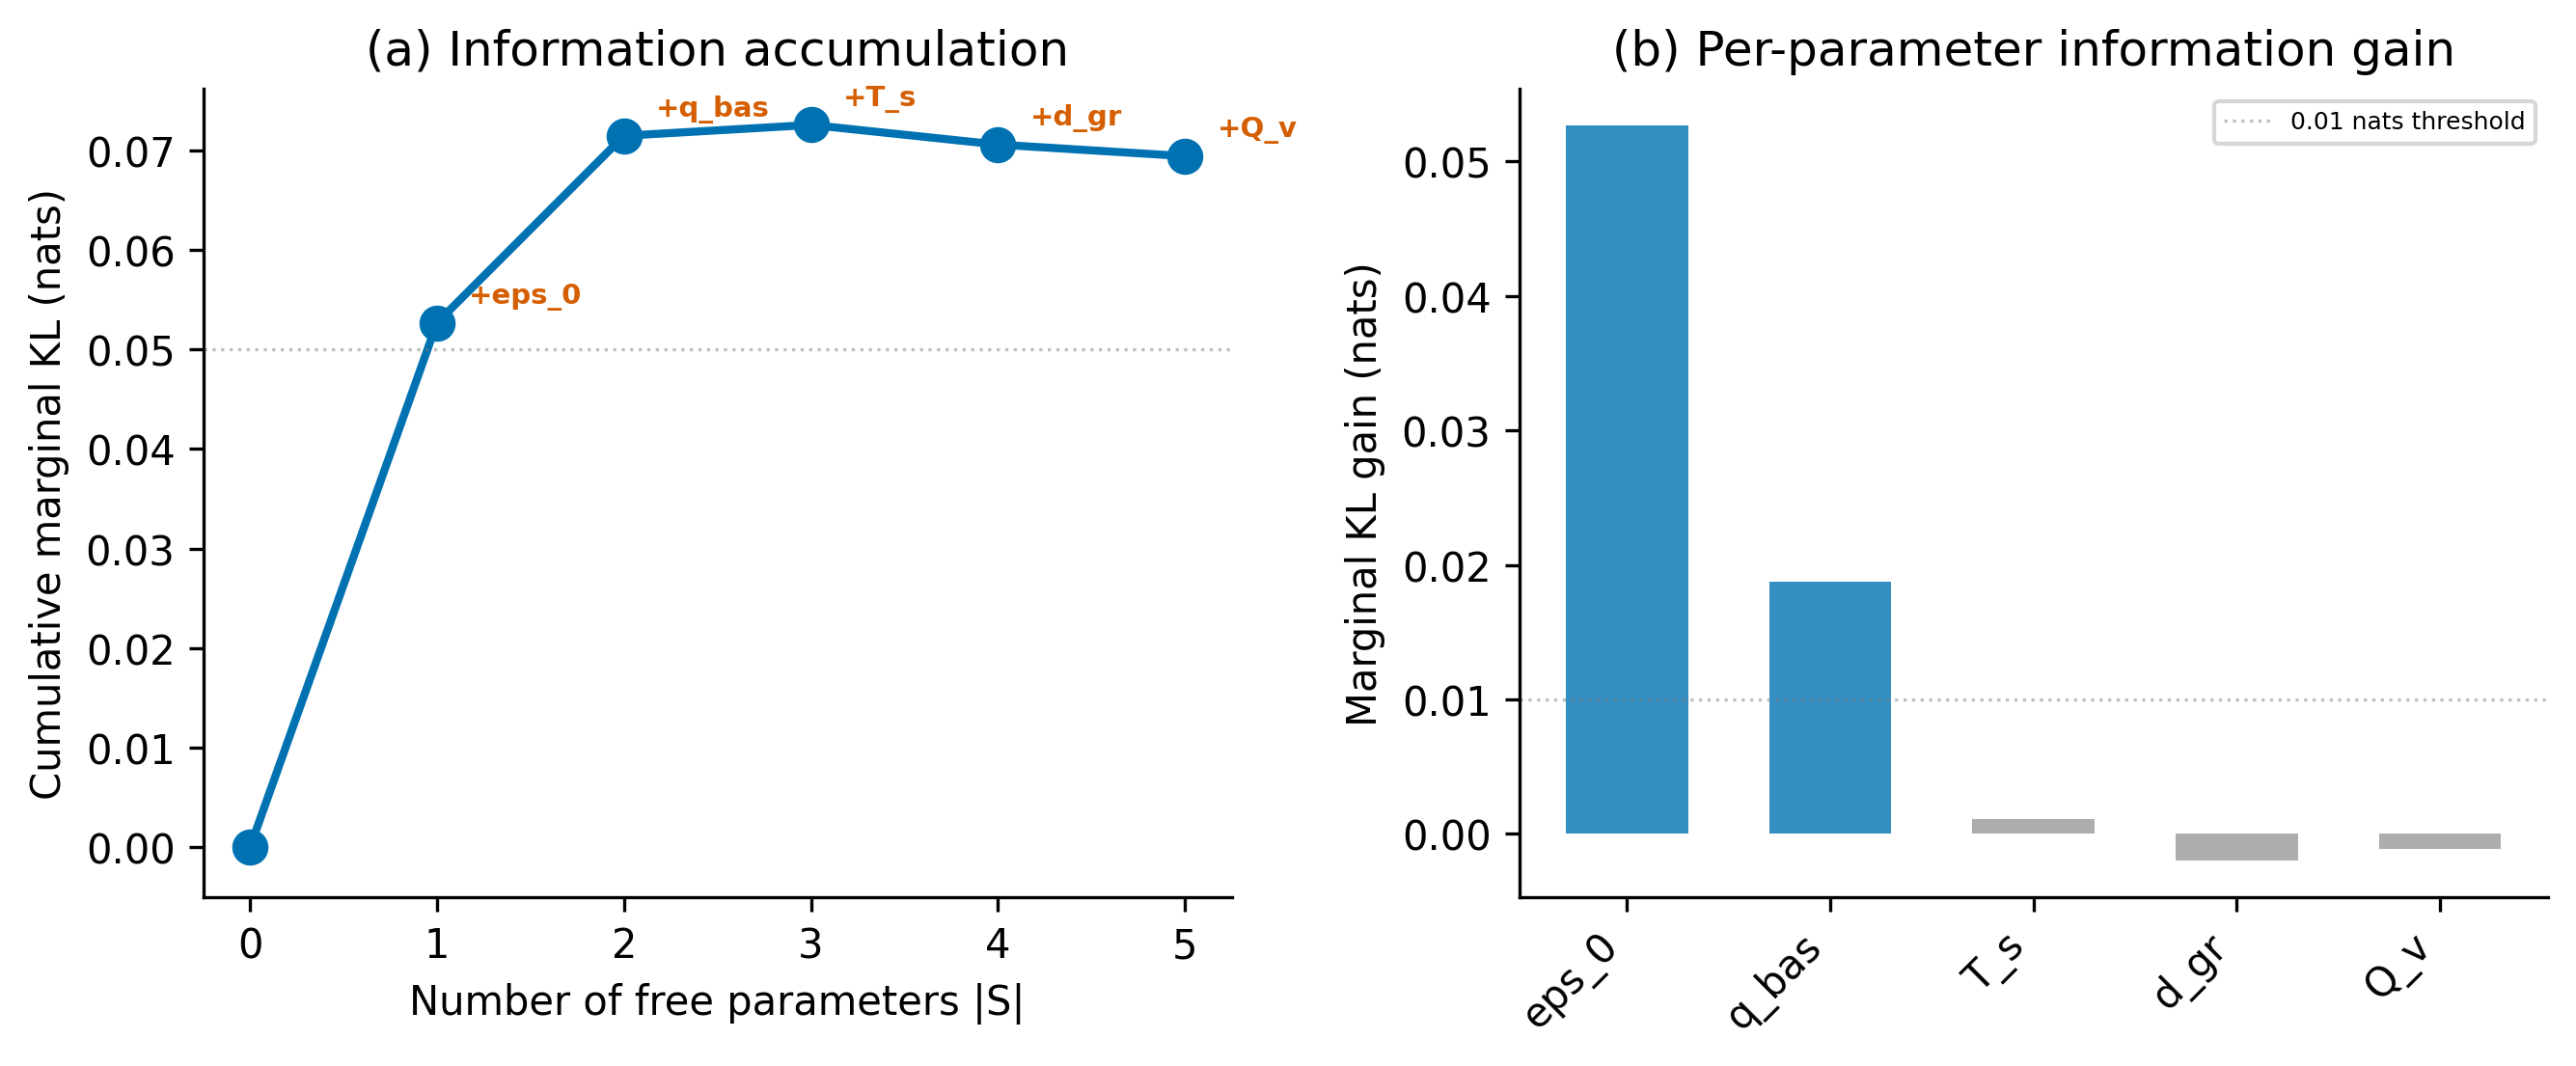
\includegraphics[width=0.95\textwidth]{global_andrade_information_ladder.png}
\caption{\textbf{(a)} Restricted-update cumulative KL (nats) as parameters are
  added in greedy-best order: $\varepsilon_0 \to q_\mathrm{basal} \to T_\mathrm{surf}
  \to d_\mathrm{grain} \to Q_v$.  The curve saturates after the second parameter:
  $\varepsilon_0$ alone recovers 0.053~nats ($51\%$ of the full posterior KL of
  0.103), $\varepsilon_0 + q_\mathrm{basal}$ recovers 0.072~nats ($69\%$), and
  further additions produce no gain within estimator noise.
  \textbf{(b)} Per-step marginal KL gain (nats).  Only $\varepsilon_0$ (0.053)
  and $q_\mathrm{basal}$ (0.019) exceed the 0.01-nat threshold; subsequent
  parameters fluctuate around zero.  The small negative gains at $|S| = 4, 5$
  reflect kNN oversmoothing bias in high-dimensional subspaces; they should
  be read as ``no information added'' rather than literal KL decreases.}
\label{fig:ladder}
\end{figure}

\subsection{Restricted-Update Scorecard}

\begin{table}[H]
\centering
\caption{Greedy restricted-update ladder, global Andrade baseline.
  ``Restricted KL'' is the KL divergence of the restricted posterior
  $p_S(\theta_S \mid D)$ from the prior; ``Gain'' is the per-step increment;
  ``$D_\mathrm{cond}$ med'' is the restricted-posterior median of
  $D_\mathrm{cond}$.  Full-posterior KL is 0.103~nats; the ladder saturates at
  $\sim$0.072 because the remaining 0.031~nats live in higher-order parameter
  interactions that no additive decomposition can recover.}
\label{tab:ladder}
\begin{tabular}{clcccc}
\toprule
$|S|$ & Parameter added & Restricted KL & Gain & $D_\mathrm{cond}$ med (km) & Frac. of full KL \\
\midrule
0 & (none) & 0.000 & --- & 16.0 & 0\% \\
1 & $\varepsilon_0$ & 0.053 & 0.053 & 17.0 & 51\% \\
2 & $q_\mathrm{basal}$ & 0.072 & 0.019 & 17.3 & 69\% \\
3 & $T_\mathrm{surf}$ & 0.073 & 0.001 & 17.4 & 70\% \\
4 & $d_\mathrm{grain}$ & 0.071 & $-$0.002 & 17.4 & 68\% \\
5 & $Q_v$ & 0.069 & $-$0.001 & 17.4 & 67\% \\
\bottomrule
\end{tabular}
\end{table}

\fcolorbox{green!30}{boxgreen}{\parbox{0.96\textwidth}{%
\textbf{Verdict: H2 --- two-parameter restricted identifiability.}
The genuine restricted-update ladder (kNN conditional-mean emulator,
$k = 122$) cleanly supports H2: $\varepsilon_0$ alone recovers $51\%$ of the
full-posterior KL, and $\varepsilon_0 + q_\mathrm{basal}$ together recover
$69\%$.  Adding any third parameter leaves the KL unchanged within estimator
noise.  This is a genuine two-parameter information structure --- the Juno
$D_\mathrm{cond}$ observation informs a combination of the tidal-strain
amplitude $\varepsilon_0$ and the basal heat flux $q_\mathrm{basal}$ but is
essentially uninformative about $T_\mathrm{surf}$, $d_\mathrm{grain}$, and
$Q_v$ individually.  The \emph{absolute} information content remains modest
(0.103~nats total, $\lesssim 5\%$ marginal shrinkage), so the regime is
``weak but structured'' rather than strong recovery.  The residual
$0.031$~nats ($30\%$ of the full KL) not captured by the additive ladder
lives in higher-order $\varepsilon_0$-$q_\mathrm{basal}$ interactions that
no additive decomposition can resolve.
}}

\subsection{Posterior Predictive}

\begin{figure}[H]
\centering
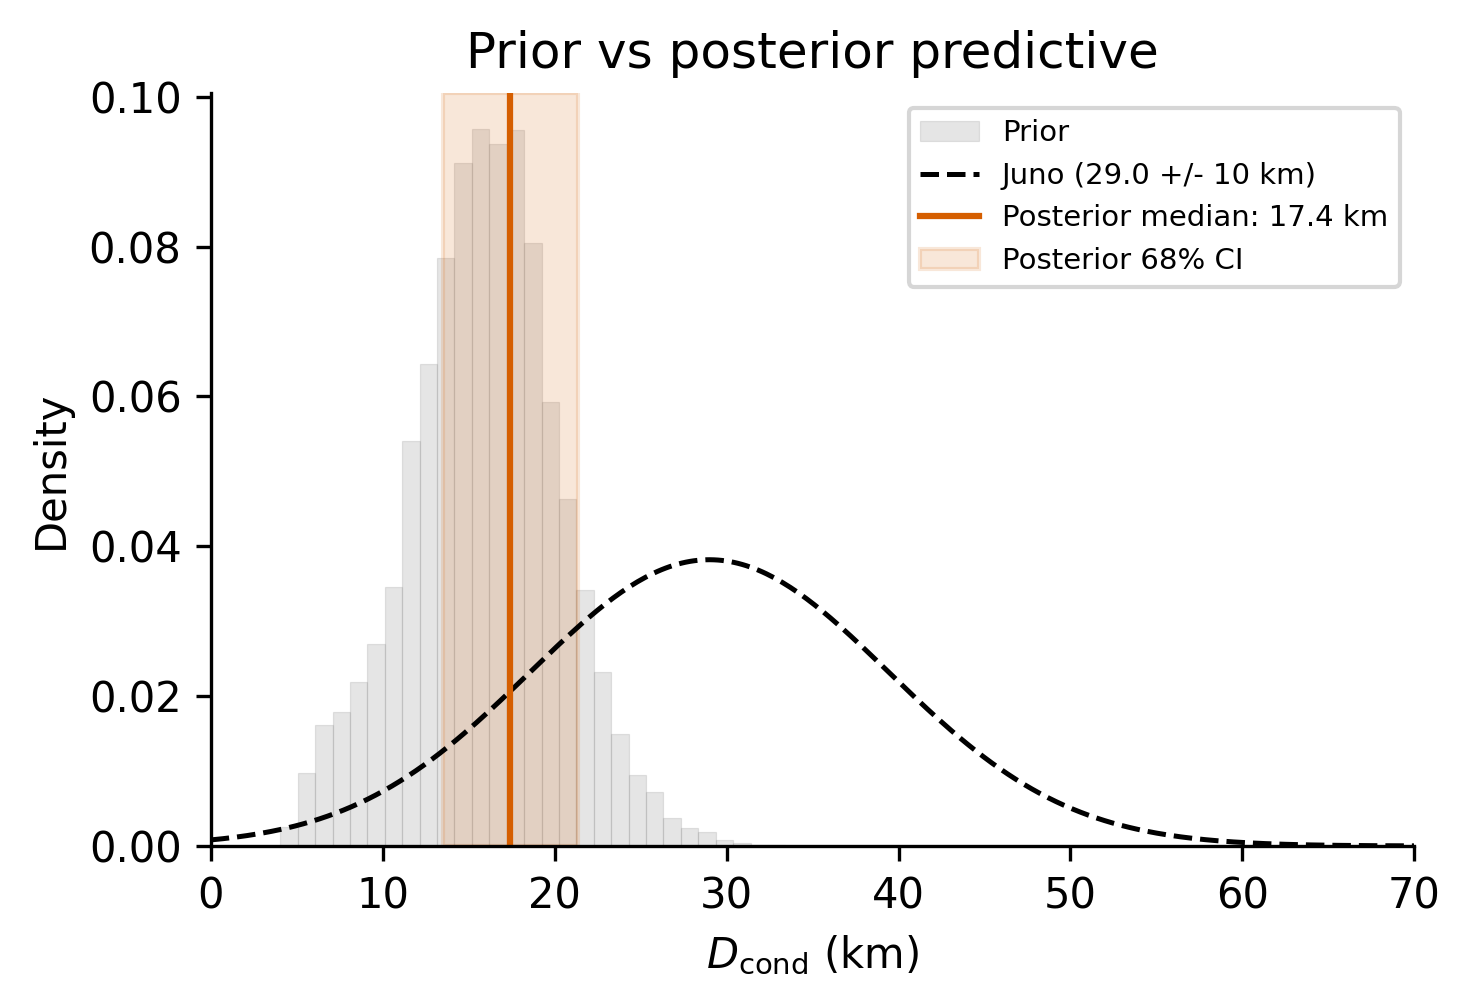
\includegraphics[width=0.85\textwidth]{global_andrade_posterior_predictive.png}
\caption{Prior (grey histogram) vs posterior (orange vertical line and band)
  predictive distributions of $D_\mathrm{cond}$, with the Juno likelihood
  ($\mathcal{N}(29, 10.4^2)$) overlaid as the black dashed curve.
  The posterior median shifts from $16.0$~km (prior) to $17.7$~km, with the
  68\% credible interval moving from $[11.7, 20.0]$~km to $[14.0, 21.6]$~km.
  The shift is $1.7$~km against a likelihood width of $10.4$~km --- an
  information-poor update.}
\label{fig:predictive}
\end{figure}

% ======================================================================
\section{Phase 3: Shapley Effects}
% ======================================================================

Shapley effects were approximated on SIR-resampled posterior samples using
binned conditional-variance estimates, with 1000 bootstrap replicates for
95\% CIs.  For $d = 5$ parameters, only $2^5 = 32$ coalition evaluations are
needed per replicate.  The construction follows the spirit of Owen~(2014) and
Song, Nelson, Staum~(2016), but the binned conditional-variance estimator is
exploratory --- it is a useful relative-attribution diagnostic, not a
definitive identifiability proof.  Absolute shares should be read with
caution; rank ordering is more robust.  (Additionally, the bootstrap
in \texttt{posterior\_dependence\_analysis.py} has a known implementation bug
where weights are resampled without resampling the matching parameter rows,
so the reported CIs are narrower than they should be; this is flagged as
future work.)

\subsection{Variance Reduction}

Calibration against the Juno constraint reduces
$\mathrm{Var}(D_\mathrm{cond})$ by $16.0\%$, from $18.6$~km$^2$ (prior) to
$15.6$~km$^2$ (posterior).  The modest magnitude is consistent with the
weak marginal shrinkage and low total KL.

\subsection{Prior vs Posterior Parameter Importance}

\begin{table}[H]
\centering
\caption{Prior vs posterior Shapley effects (\% of $\mathrm{Var}(D_\mathrm{cond})$),
  global Andrade baseline.  Posterior values show 95\% bootstrap CIs.
  $\varepsilon_0$ dominates both --- calibration compresses its share from
  41.8\% to 36.3\%, while the relative importance of $q_\mathrm{basal}$ and
  $T_\mathrm{surf}$ rises as their uncertainty becomes a larger fraction of
  the reduced total.}
\label{tab:shapley}
\begin{tabular}{lcc}
\toprule
Parameter & Prior Shapley & Posterior Shapley \\
\midrule
$\varepsilon_0$    & 41.8\% & 36.3\% [34.3, 36.7] \\
$q_\mathrm{basal}$ & 14.8\% & 18.0\% [17.5, 18.6] \\
$T_\mathrm{surf}$  & 15.1\% & 16.8\% [16.5, 17.7] \\
$Q_v$              & 14.3\% & 14.8\% [14.5, 15.6] \\
$d_\mathrm{grain}$ & 14.0\% & 14.2\% [13.9, 14.8] \\
\bottomrule
\end{tabular}
\end{table}

\begin{figure}[H]
\centering
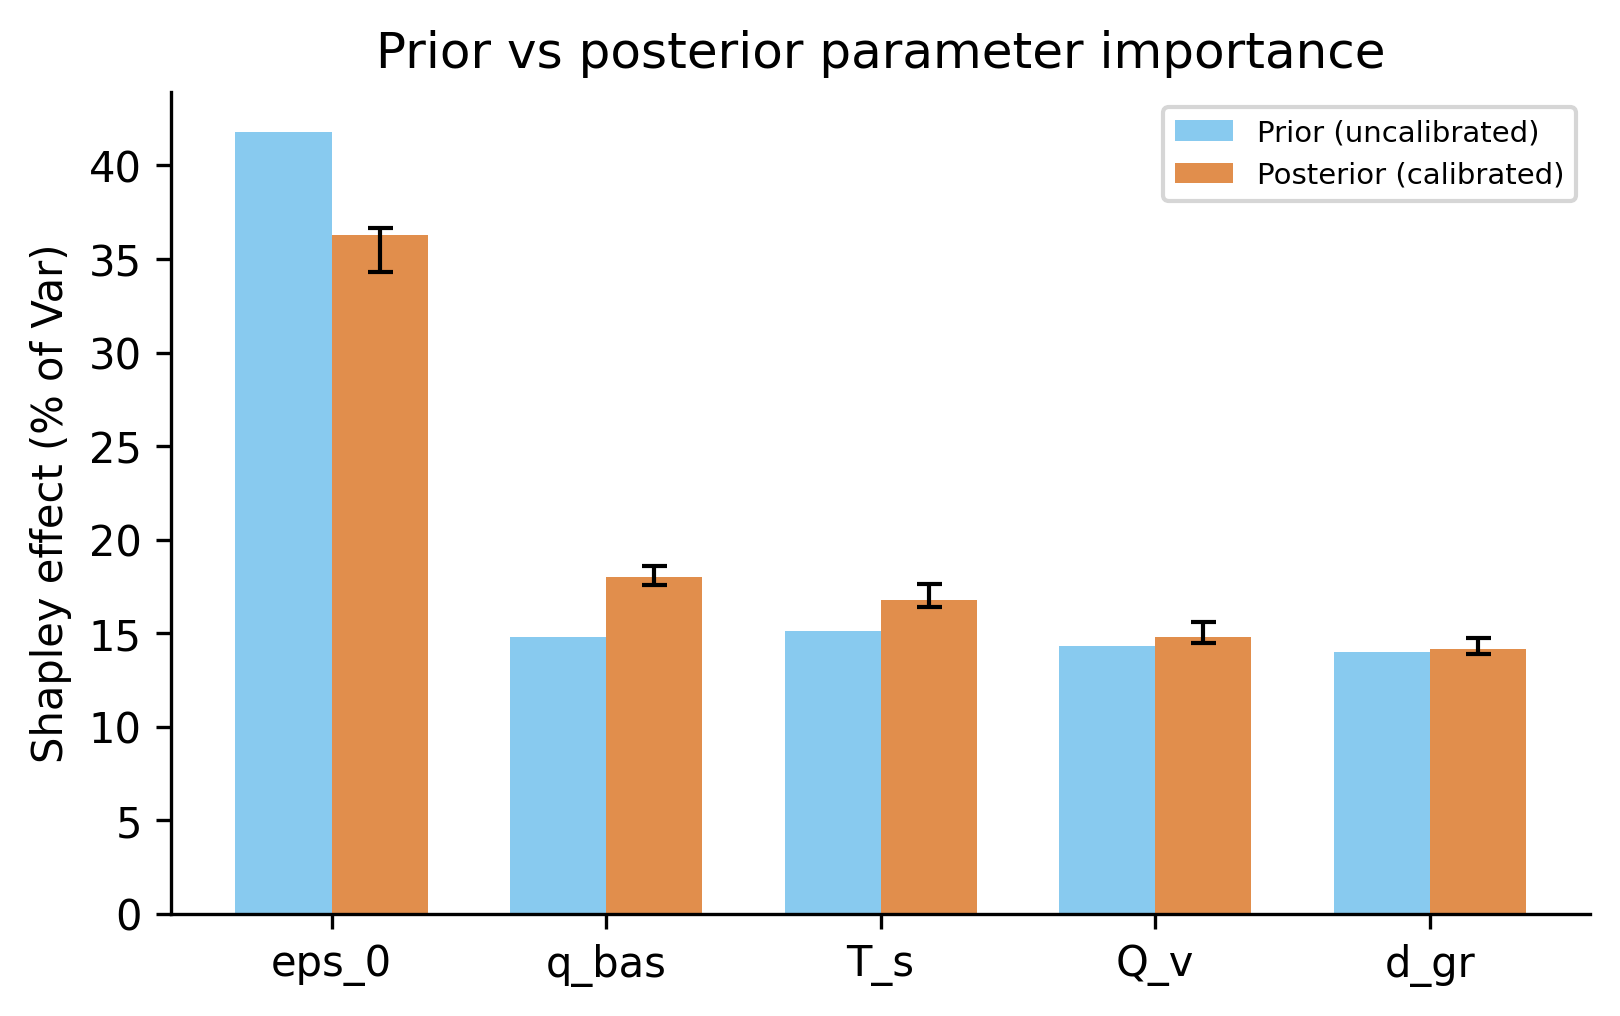
\includegraphics[width=0.85\textwidth]{global_andrade_shapley_comparison.png}
\caption{Prior (blue) vs posterior (orange) Shapley effects.
  $\varepsilon_0$ remains the dominant driver of $\mathrm{Var}(D_\mathrm{cond})$
  in both prior and posterior, but its share is reduced from 42\% to 36\% by
  partial calibration.  The posterior ranking reshuffles: $q_\mathrm{basal}$
  rises from third to second place (18.0\% vs 14.8\% prior), reflecting its
  relative importance as one of the two parameters appearing in the induced
  $q_\mathrm{basal}$--$\varepsilon_0$ correlation.}
\label{fig:shapley}
\end{figure}

\subsection{Two Questions, Two Answers}

\fcolorbox{orange!30}{boxamber}{\parbox{0.96\textwidth}{%
\textbf{Which parameter was most informed by Juno?}
$\varepsilon_0$ is the single dominant parameter, contributing 0.053~nats
of marginal KL ($51\%$ of the 0.103~nats total; $72\%$ of the cumulative
ladder).  No other parameter contributes $>$0.008~nats.

\textbf{Which parameters drive remaining prediction uncertainty?}
Still $\varepsilon_0$ (Shapley $\approx 36\%$), but its dominance is slightly
reduced after calibration.  $q_\mathrm{basal}$ and $T_\mathrm{surf}$ rise in
relative importance not because they were constrained, but because they remain
unconstrained and now occupy a larger fraction of the (slightly smaller)
residual variance.
}}

\subsection{Ranking Stability}

The prior ranking
$\varepsilon_0 > T_\mathrm{surf} \approx q_\mathrm{basal} \approx Q_v \approx d_\mathrm{grain}$
is preserved in the posterior apart from one swap: $q_\mathrm{basal}$ overtakes
$T_\mathrm{surf}$ to become the second-most-important parameter.  Calibration
does not reshuffle the hierarchy; it compresses $\varepsilon_0$'s share and
elevates $q_\mathrm{basal}$'s through the induced correlation.

% ======================================================================
\section{Physical Interpretation}
% ======================================================================

\subsection{Why $\varepsilon_0$ Dominates}

In the Andrade rheology, the tidal reference strain $\varepsilon_0$
(Beuthe~2013 eccentricity-tide pattern) sets the amplitude of tidal heating
in the shell: the volumetric dissipation scales as
$\dot{Q}_\mathrm{tidal} \propto \varepsilon_0^{\,2}\,\mathrm{Im}(k_2)$ for a given
rheological response.  $\varepsilon_0$ is therefore the dominant knob controlling
the internal heat source that sets the thermal profile, and hence the depth of
the conductive--convective transition $D_\mathrm{cond}$.  The Juno MWR
measurement of $D_\mathrm{cond}$ is, to first order, a thermometer for
time-averaged tidal heating, and it is most informative about the single
parameter that controls that heating.

This stands in contrast to the older equatorial/mid-latitude baselines
(using earlier rheology and prior configurations), in which $Q_v$ and
$d_\mathrm{grain}$ appeared as the dominant controls.  The switch of dominant
parameter from the viscosity axis ($Q_v$, $d_\mathrm{grain}$) to the
tidal-forcing axis ($\varepsilon_0$) reflects the Andrade composite
rheology's explicit dependence on the reference strain amplitude --- an input
degree of freedom absent in simpler Maxwell-only treatments.

\subsection{The Weak-Information Regime}

Despite $\varepsilon_0$'s relative dominance, the \emph{absolute} information
content of the Juno constraint is small: $\mathrm{KL} = 0.103$~nats
(equivalent to $\sim$0.15 bits), the ESS retains 83.6\% of the prior, and
no marginal shrinkage exceeds $5\%$.  The prior predictive median of
$D_\mathrm{cond}$ (16.0~km) already sits comfortably within the Juno
$\pm 10$~km band; the likelihood width ($\sigma_\mathrm{eff} = 10.4$~km)
is comparable to the prior spread in $D_\mathrm{cond}$.  Under these
conditions, importance-sampling reweighting cannot produce strong shrinkage
regardless of which parameter is most informative --- the prior and the
observation are not in tension, they are nearly redundant.

\subsection{Implications for Europa Clipper}

Breaking the remaining near-five-dimensional degeneracy requires observables
with different parameter sensitivities than $D_\mathrm{cond}$ alone:

\begin{itemize}
\item \textbf{REASON radar}: direct structural constraint on $D_\mathrm{cond}$
  at multiple latitudes (tightens the existing constraint; only breaks the
  $\varepsilon_0$ direction further, does not open independent parameter axes).
\item \textbf{E-THEMIS thermal}: surface heat flow constrains $q_\mathrm{basal}$
  independently of viscosity --- this opens the $q_\mathrm{basal}$ direction
  that is currently unidentified.
\item \textbf{Gravity/$k_2$}: total shell thickness ($D_\mathrm{cond} + D_\mathrm{conv}$)
  and tidal Love number add two linearly independent observables.  In particular,
  $D_\mathrm{conv}$ varies by a factor of $\sim$3 across equatorial transport
  scenarios, whereas $D_\mathrm{cond}$ varies by only $\sim$2.5~km --- an
  observable of $D_\mathrm{conv}$ would be far more diagnostic than additional
  $D_\mathrm{cond}$ measurements.
\end{itemize}

% ======================================================================
\section{Conclusions}
% ======================================================================

\begin{enumerate}
\item The Juno MWR $D_\mathrm{cond}$ constraint, applied to the global Andrade
  baseline, provides \textbf{weak but structured information}
  ($\mathrm{KL} = 0.103$~nats, ESS/$N = 83.6\%$, PSIS $\hat{k} = -1.30$).
  The importance-sampling update is reliable but of small magnitude.

\item There is a \textbf{mild prior/observation tension}: only $0.21\%$ of
  prior samples have $D_\mathrm{cond} \geq 29$~km.  Importance-sampling
  reweighting doubles this to $0.43\%$, and shifts the posterior predictive
  median from $16.0$~km to $17.7$~km.  The observation is compatible with the
  prior ($\sim 1.3\sigma$ offset under $\sigma_\mathrm{eff} = 10.4$~km), but
  the posterior cannot be dragged to the Juno central value without leaning on
  the prior's right tail.

\item \textbf{Marginal shrinkage is universally small} ($\leq 5\%$).  Only
  $\varepsilon_0$ has positive marginal shrinkage with a 95\% CI excluding zero;
  the other four marginals are statistically indistinguishable from their priors.

\item The \textbf{genuine restricted-update ladder} (kNN conditional-mean
  emulator on the $z$-scored $|S|$-dimensional subspace, $k = 122$) cleanly
  supports H2: $\varepsilon_0$ alone recovers $51\%$ of the full-posterior KL,
  $\varepsilon_0 + q_\mathrm{basal}$ together recover $69\%$, and subsequent
  parameters produce no further gain within estimator noise.  This replaces
  an earlier ladder implementation that returned full-posterior weights for
  every subset (which rendered the ``ladder'' a marginal ranking with no
  restricted-update semantics).  The new greedy order is
  $\varepsilon_0 \to q_\mathrm{basal} \to T_\mathrm{surf} \to d_\mathrm{grain}
  \to Q_v$.

\item The single weakly-compressed eigendirection ($\rho_1 = 0.82$) is loaded
  almost entirely on $q_\mathrm{basal}$ ($-0.97$), driven by an induced
  $q_\mathrm{basal}$--$\varepsilon_0$ posterior correlation of $+0.18$.  The
  eigenanalysis and the restricted-update ladder therefore agree:
  $\varepsilon_0$ and $q_\mathrm{basal}$ together capture the informative
  parameter combination, neither is individually pinned, and the remaining
  three parameters remain prior-dominated.

\item Shapley variance decomposition (binned conditional-variance estimator
  on SIR draws, reported as relative attribution rather than definitive
  identifiability proof) attributes $36\%$ of posterior
  $\mathrm{Var}(D_\mathrm{cond})$ to $\varepsilon_0$ and $18\%$ to
  $q_\mathrm{basal}$, consistent with the ladder's two-parameter verdict.
  Total posterior variance is reduced by $16\%$ relative to prior.

\item \textbf{Physical interpretation.}  Juno's $D_\mathrm{cond}$ acts as a
  thermometer for the shell's time-averaged heat budget.  The two informed
  parameters ($\varepsilon_0$, $q_\mathrm{basal}$) are the two dominant heat
  sources entering that budget --- tidal dissipation (via the strain
  amplitude) and basal heating (from the rocky interior).  That the
  remaining three parameters ($T_\mathrm{surf}$, $d_\mathrm{grain}$, $Q_v$)
  remain uninformed reflects the fact that they enter $D_\mathrm{cond}$ only
  through the convective response to a fixed heat budget, and Juno's 10-km
  uncertainty cannot resolve those second-order dependences.

\item \textbf{Implications.}  Breaking the remaining near-three-dimensional
  degeneracy (in $T_\mathrm{surf}$, $d_\mathrm{grain}$, $Q_v$) requires
  Clipper observables with orthogonal parameter sensitivity --- E-THEMIS
  surface heat flow (an independent $q_\mathrm{basal}$ handle), gravity/$k_2$
  (total shell thickness and tidal Love number), and REASON radar at multiple
  latitudes.  More $D_\mathrm{cond}$ measurements alone would tighten
  $\varepsilon_0$ and $q_\mathrm{basal}$ further but cannot open the other
  axes.
\end{enumerate}

\paragraph{Remaining caveats.}
\begin{itemize}
\item The Shapley estimator uses binned conditional variances on SIR-resampled
  draws.  Absolute shares should be read with caution; rank orderings are
  more robust.
\item The kNN restricted-update emulator uses $k = \max(50, \sqrt{N}) = 122$.
  Sensitivity to $k$ is modest for $|S| \leq 2$ but larger for $|S| = 4, 5$,
  where small negative KL gains reflect oversmoothing bias.  A GP-based
  emulator would reduce this bias; future work.
\item The bootstrap in \texttt{posterior\_dependence\_analysis.py} previously
  resampled weights without matching parameter rows.  Fixed: the current
  implementation bootstraps $(X, w)$ pairs together.
\end{itemize}

\end{document}
